\documentclass{article}
\usepackage{graphicx}
\graphicspath{ {graphs/} }
\begin{document}
\begin{titlepage}
    \begin{center}
        \vspace*{1cm}
        
        \Huge
        \textbf{Reconstruction of Charge Number of Heavy Cosmic Rays using Cherenkov Light}
        
        \LARGE
        
        \vspace{1cm}
        
        \textbf{Robert Stein}\\
        \textbf{CID 00819615}
        
        \vspace{1cm}
        
\includegraphics[width=0.4\textwidth]{Imperial_College_London_logo} 
        \hspace{0.5cm}
        
\includegraphics[width=0.4\textwidth]{hamburglogo}
        
        \vspace{1cm}
        
        Supervisor: Professor Dieter Horns
        
        \large
        \vspace{1.0cm}
        
        A thesis presented for the degree of\\
        \textbf{Master in Science}
        
        \vspace{0.5cm}

        Physics Department\\
        Imperial College London
        
        \vspace{0.5cm}
        
        \today
        
    \end{center}
\end{titlepage}
\section*{Abstract}
Between impact with the upper atmosphere and decay into a charged particle shower, heavy cosmic ray elements such as Iron emit Cherenkov Light at an angle determined by the Refractive Index of the air and the energy per nucleon. This direct Cherenkov Light forms a characteristic circular light distribution on the Earth's surface with an intensity proportional to the square of the cosmic ray charge. A new method has been developed to reconstruct this charge number, by fitting the received Cherenkov Photons to the characteristic Lateral Photon Distribution. The expected performance for various existing and planned installations will be discussed.

\section*{Zusammenfassung}
Between impact with the upper atmosphere and decay into a charged particle shower, heavy cosmic ray elements such as Iron emit Cherenkov Light at an angle determined by the Refractive Index of the air and the energy per nucleon. This direct Cherenkov Light forms a characteristic circular light distribution on the Earth's surface with an intensity proportional to the square of the cosmic ray charge. A new method has been developed to reconstruct this charge number, by fitting the received Cherenkov Photons to the characteristic Lateral Photon Distribution. The expected performance for various existing and planned installations will be discussed.
\newpage
\tableofcontents
\newpage
\section{Introduction}
There are numerous Telescope Arrays which image the Cherenkov Light emitted by Cosmic Rays in the atmosphere, including the HESS, Magic and Veritas Experiments. All such Imaging Atmospheric Cherenkov Telescopes (IACTs) rely on Hillas Analysis for event reconstruction.Hillas Analysis extracts parameters from each of the camera images in order to reconstruct the events. However, heavy blurring of the events by atmospheric effects means that resolution of reconstruction  is very poor. For a typical Iron Nucleus event \cite{hess07}, the core position resolution is roughly $d \approx 20 m $, and the charge would be reconstructed as \[Z \approx 26 \pm 5 \]

Cosmic Rays that are imaged by these telescopes have energies between $13 $TeV and $200 $TeV. At present, no study of the relative abundance of different cosmic ray elemental abundances exists, although it could provide important clues regarding the mechanism of Cosmic Ray formation and propagation in the galaxy. Unfortunately, current charge resolution from Hillas Analysis is not small enough to undertake such a study.

Instead of Hillas Analysis, we consider a new method for event reconstruction, in which we fit the known Direct Cherenkovn (DC) Light observed by each telescope to a characteristic Lateral Photon Distribution (LPD) function. This new technique is valid both for currently running experiments, as well as planned experiments such as the Cherenkov Telescope Array (CTA). It uses only the information from the DC Pixel identified in the shower images.

A theoretical study by Kieda in 2001 \cite{kieda01} suggested that for a core position resolution of $d \approx 5 $ m , we could expect to see a charge resolution of $ \sigma_{Z} \approx 1 $ for elements of $Z = 20$ or higher. In this case the core resolution would be the limiting value. Thus, if the LPD method can achieve this core position resolution, then charge resolution will become sufficiently good enough to extract the abundances of the different Cosmic Ray Elements. This the prime motivation for the new LPD technique.

\section{Lateral Photon Distribution Method}
In order to reconstruct events using the LPD method, we require the Energy of the Cosmic Ray lie in the saturated region, and that the event can be seen by at least 4 telescopes. These restrictions confine us to Cosmic Rays with specific characteristics.

\subsection{Cherenkov Light Emission}
Cosmic Rays follow a well-defined power law where $ \frac{dN_{E}}{dt} \propto E^{-\gamma} $ and experimentally $ \gamma = 2.7 \pm ? $. Consequently higher energy Cosmic Rays are heavily suppressed. 

The energy Threshold as a function of height is illustrated in

Once a Cosmic Ray crosses the Threshold Energy, it will begin emitting Cherenkov Light, and will stop emitting Cherenkov Light when it first interacts at a height $h$. For a given Telescope Array altitude above sea level, simple trigonometry yields:
\[ Radius(height = altitude_{array}) = \tan (\theta_{C}(h)) \times (h - altitude_{array})\]
As the Refractive Index of the Earth increases as height decreases, the angle $\theta_{C}$ increases with decreasing height. Thus the upper earlier emission contributes to the inner LPD, while the later emission contributes to the high-radius LPD. 

In figure Y, we see ground emission radius as a function of height. It is clear that the high-radius emission, (occurring near the first interaction region) is virtually unchanged for different Energies. We deem this to be 'saturated emission'.

\subsection{Nuclear Charge}
In figure Z we see that the height of the 'signal' LPD varies with \[ \rho_{DC}  = f(r) \times Z^{2}\]

Thus the height of the LPD is proportional to the charge of the Cosmic Ray, enabling the Charge to be determined from the DC emission. This is the basis for charge reconstruction in the LPD method.

\subsection{Iterative Log Likelihood Minimisation}
In order to reconstruct an event, we need to find the x/y core position, the Energy per Nucleon, the first interaction height and the charge. However, if one telescope in a five-telescope array does not observe DC light, this data point can be used to constrain the core position. Thus, for the LPD method to be applied, we require a minimum of five telescopes, four or more of which must image the DC light.

We consider the amount of DC light that each telescope receives to be Poissonian \[  P_{i} ( N_{i, Received} \mid X, Y, Z, height, Epn )  =  \frac{ e^{- \lambda_{i} } \times \lambda_{i} ^{N_{i}} }{N_{i}!} \]

In order to reduce computing time, we can use Stirling's Approximation $ln( N! )  \approx  N ln(N) - N + \frac{1}{2} ln(2 \pi N)$. Pure night sky background requires that there be more that X photons in a DC pixel, and for this Stirling's Approximation has an error of just Y?. We then minimise the Log Likelihood function \[ - Ln(L) = - \sum_{i=1}^{n} [P_{i}] \approx  \sum_{i=1}^{n} [\lambda _{i} - N_{i} ln(\lambda _{i}) + N_{i} ln(N_{i}) - N_{i} + \frac{1}{2} ln(2 \pi N_{i})]  \]
where n is the total number of telescopes in the array.

Unfortunately, as a result of varying Threshold Energies and the sharp drop in the LDF above the maximum radius, the Log likelihood is discontinuous in many places. Consequently, a Minuit-type minimisation algorithm will only be able to find a local minimum near the starting values for the fit parameters.


\section{HESS-type Event Reconstruction}

\subsection{First Interaction Height}
Cosmic Rays survival in from the top of the atmosphere follows an exponential decay with the number of 'interaction lengths' passed. The interaction length is dependent on the interaction cross section, which increases with density. Thus the number of interaction lengths increases exponentially as height decreases . 

The resultant decays occur most often at a height of $h \approx 40 \pm 10$ km. However, when the HESS layout is simulated, the 4 telescope events have a mean height of $h \approx 24 \pm 4$ km, as shown in \ref{fig:Height Statistics}.

\begin{figure}
\begin{center}
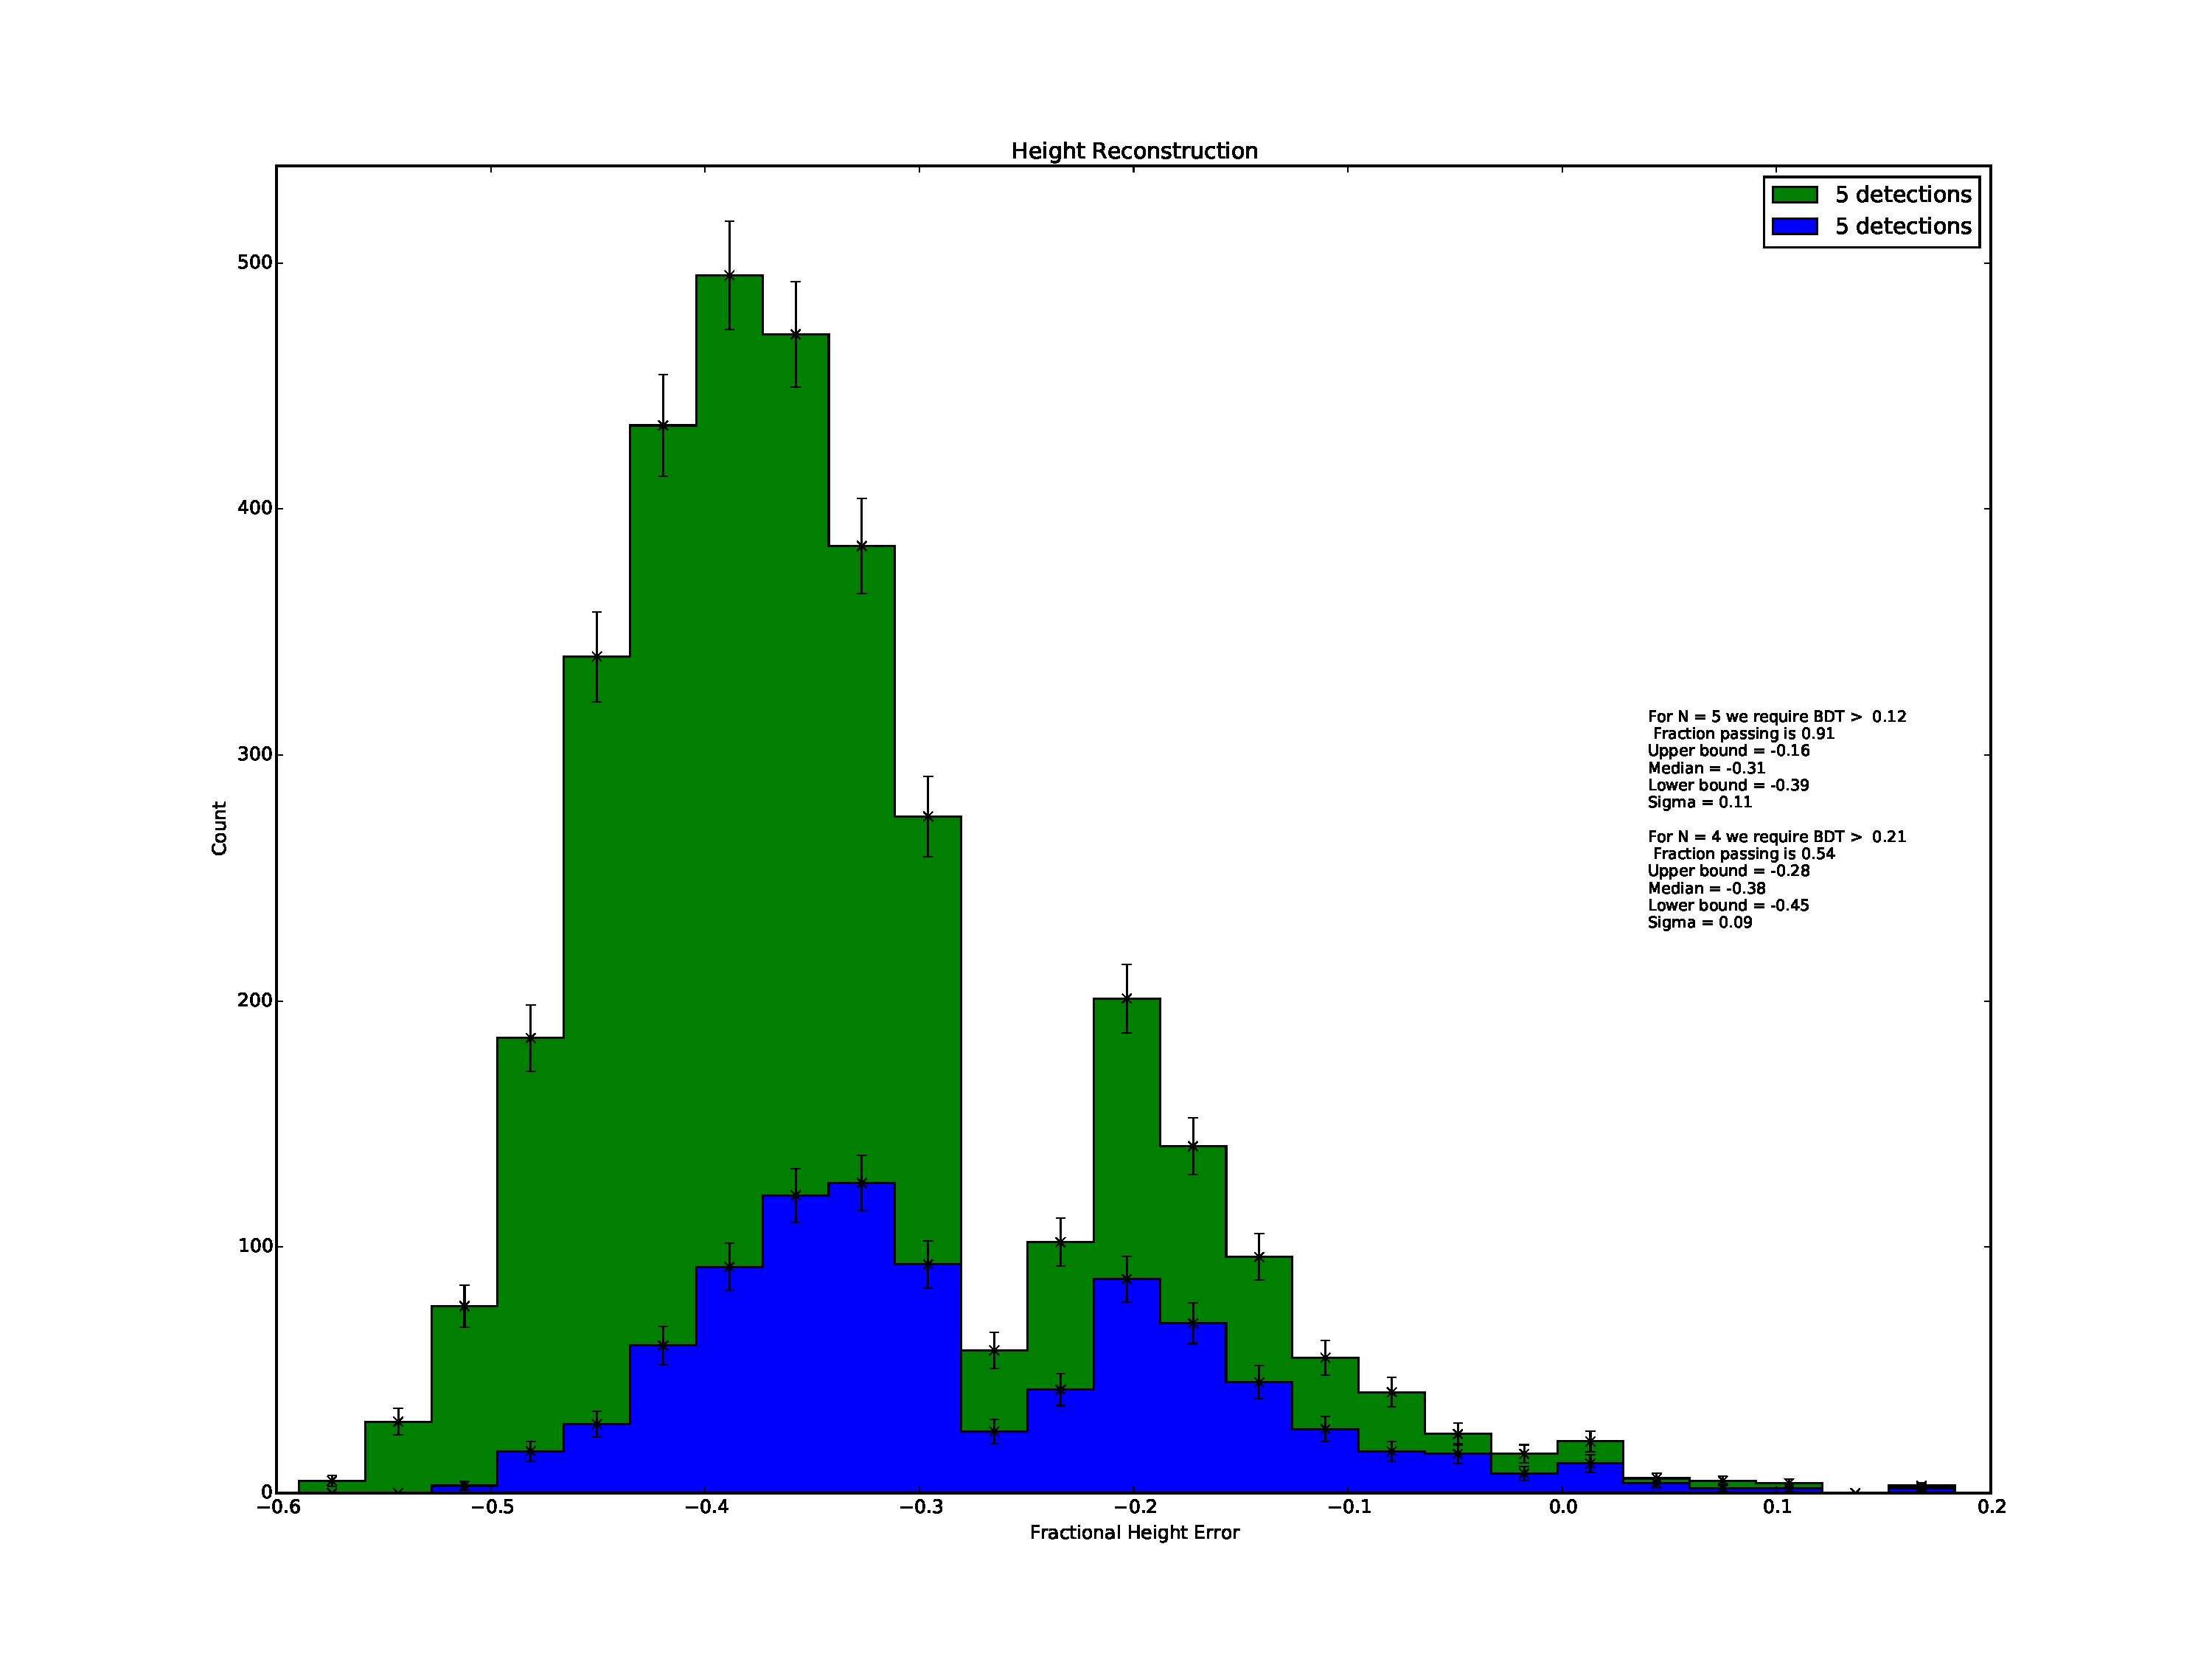
\includegraphics[height=0.9\textheight]{height}
\caption{The integrated interaction lengths increases as height decreases. Thus the decay probability follows a exponentially increasing distribution. The first interaction height for all events peaks at around 40000m. However the mean first interaction height for 4 telescope events is 23000m}
\label{fig:Height Statistics}
\end{center}
\end{figure}

\subsection{HESS Energy saturation region}
It be like 0.7 Tev per Nucleon!

However, in the 4 telescope height region, the Cherenkov Threshold Energy is $ E_{Threshold} \approx 0.35$ TeV per Nucleon fig Y! The saturation in for these heights occurs roughly at 0.7 TeV per Nucleon or something...

\subsection{Extended Air Shower Background}
A typical HESS image is shown in \ref{fig:hess}, with the DC pixel visible. The Extended Air Shower (EAS) produced after the first interaction of the Cosmic Ray overlaps the DC pixel, leading to background in the LPD. As the Energy of the Cosmic Ray increases, the EAS speads over a larger angular area, and at smaller radii, the EAS-DC-shower direction axis contracts, leading to more overlap. Thus the background in the DC pixel increases with decreasing radius and increasing Energy. 

\begin{figure}
\begin{center}
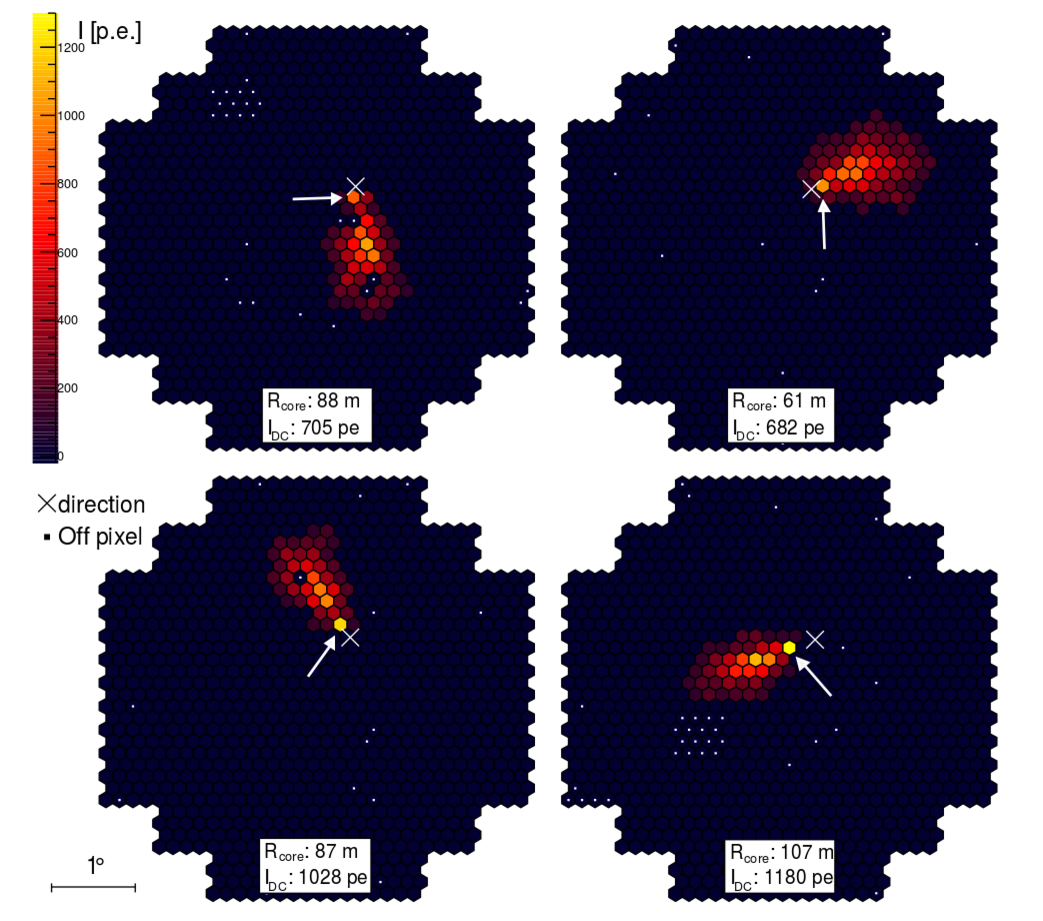
\includegraphics[width=0.9\textwidth]{hess}
\caption{A 4-camera HESS event. The shower direction is marked with a white cross, and the DC pixel is indicated with a white arrow. The shower axis passes through the shower direction, the DC pixel, and the center of the Extensive Air Shower region lying beyond the DC pixel.}
\label{fig:hess}
\end{center}
\end{figure}

In addition, we have a fixed night sky background with 7 photons $m^{-2}$. We thus parameterise the background with 
\[ \rho_{bkg}  = 7 + 5E\]
The modeled background LPD is shown in X. It begins to dominate above roughly 1 TeV per Nucleon, particularly in the case of smaller radii.

\section{Optimised Telescope Array}
NO Background!!!!!
\subsection{Count Rates}

\subsection{Saturation Region Energies}



\section{Conclusion}
End
\bibliographystyle{plain}
\bibliography{report}
\end{document}